\section{Iterated Cipher dan Jaringan Feistel}
Untuk mencapai keamanan yang tinggi, \textit{block cipher} modern menggunakan struktur \textbf{Iterated Cipher}, di mana fungsi transformasi (fungsi putaran) diterapkan berulang kali selama $r$ putaran.

\subsection{Jaringan Feistel}
Struktur yang sangat populer (digunakan pada DES) adalah \textbf{Jaringan Feistel}. Dalam struktur ini, blok data dibagi menjadi dua bagian, Kiri ($L$) dan Kanan ($R$):
\begin{align*}
L_i &= R_{i-1} \\
R_i &= L_{i-1} \oplus f(R_{i-1}, K_i)
\end{align*}
Sifat utama Jaringan Feistel adalah \textbf{reversible}. Proses dekripsi dilakukan dengan urutan putaran yang terbalik menggunakan kunci yang sama, tanpa perlu membuat fungsi dekripsi $f^{-1}$ yang terpisah.

\subsection{Pembangkitan Kunci Putaran (Key Scheduling)}
Setiap putaran dalam \textit{iterated cipher} menggunakan kunci internal yang berbeda, disebut \textbf{subkey} atau \textit{round key}. Kunci-kunci ini dibangkitkan dari kunci eksternal yang diberikan pengguna melalui proses \textit{key expansion}.

\subsection{Ukuran Blok dan Kunci}
\begin{itemize}
    \item \textbf{Ukuran Blok}: Semakin besar blok, semakin kuat efek difusinya (misal: AES menggunakan 128 bit).
    \item \textbf{Ukuran Kunci}: Semakin panjang kunci, semakin tahan cipher terhadap serangan \textit{brute force} (misal: AES-256 lebih kuat dari AES-128).
\end{itemize}






\begin{figure}[htbp]
    \centering
    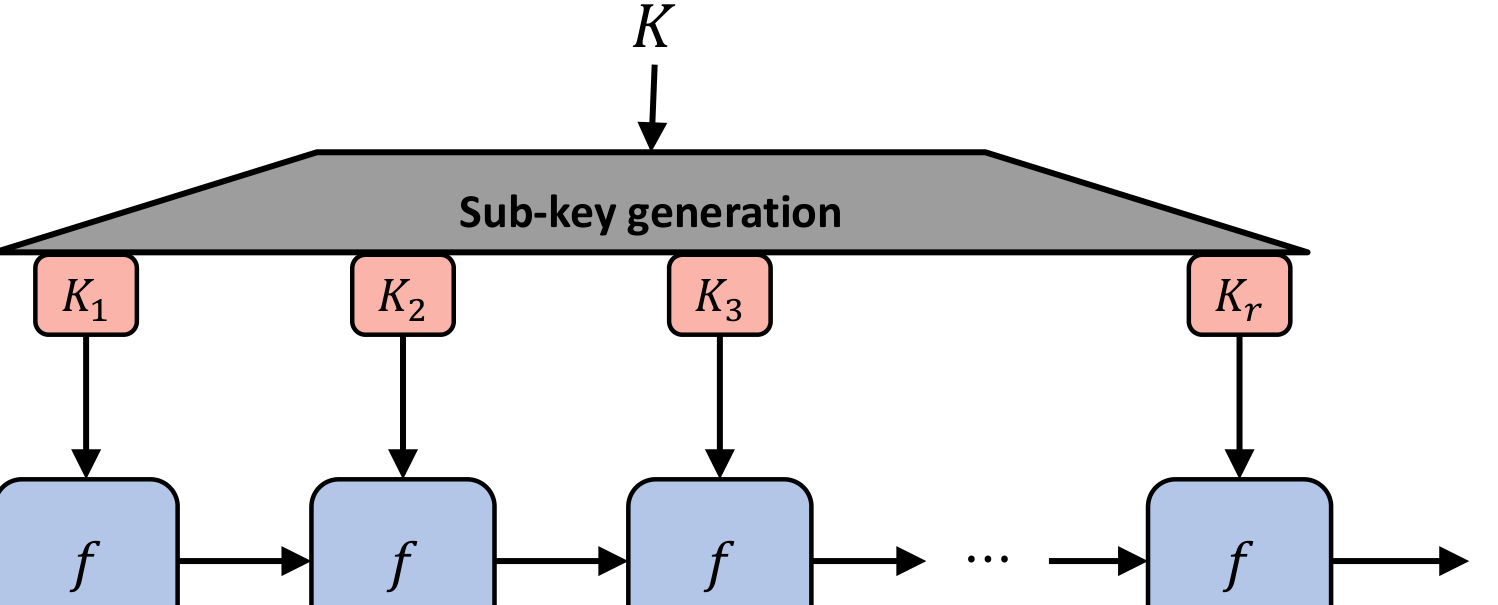
\includegraphics[width=0.85\linewidth, height=0.8\textheight, keepaspectratio]{figures/pembangkitan-subkunci.png}
    \caption{Pembangkitan subkunci: kunci utama diturunkan menjadi subkunci yang masing-masing menyuapi fungsi putaran secara berurutan}
    \label{fig:pembangkitan-subkunci}
    \sumber{Munir, \textit{IF4020 Kriptografi}, ITB.}
\end{figure}

\begin{figure}[htbp]
    \centering
    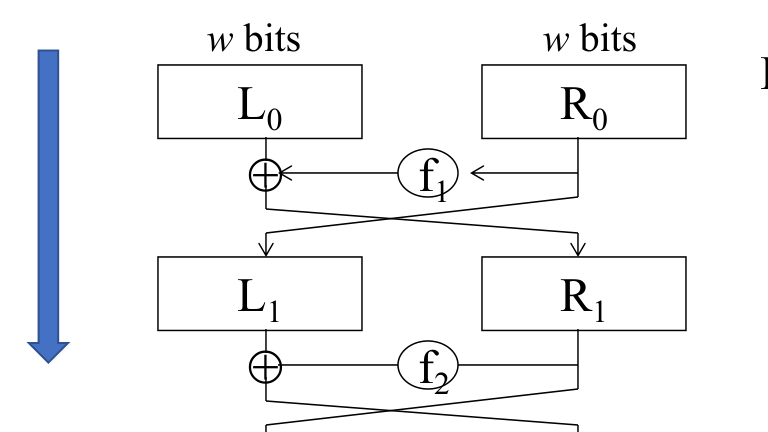
\includegraphics[width=0.8\linewidth, height=0.8\textheight, keepaspectratio]{figures/jaringan-feistel.png}
    \caption{Jaringan Feistel multi-putaran yang memperlihatkan pertukaran peran blok kiri dan kanan serta penerapan fungsi putaran pada setiap putaran}
    \label{fig:jaringan-feistel}
    \sumber{Munir, \textit{IF4020 Kriptografi}, ITB.}
\end{figure}
